\documentclass[12pt]{article}

\usepackage{sbc-template}

\usepackage{graphicx,url}

\usepackage[brazil]{babel}   
\usepackage{verbatim}
\usepackage{todonotes}
\usepackage{longtable}
\usepackage{amssymb}
\usepackage{amsmath}
\usepackage{float}
\usepackage{amsfonts}
\usepackage{color}
\usepackage{url}
\usepackage[utf8]{inputenc}  
\usepackage{paralist}
% UTF-8 encoding is recommended by ShareLaTex

     
\sloppy

\title{Estado da Arte \\Sistemas de Assistência de Direção usando \textit{Hardware} Reconfigurável}
\author{Rodolfo Labiapari Mansur Guimarães}

\address{Departamento de Computação -- Universidade Federal de Ouro Preto \\
 35.400-000 -- Ouro Preto - MG -- Brasil
 \email{rodolfolabiapari@gmail.com }
}

\begin{document} 

\maketitle

\section{Introdução}
\subsection{Problema}
% iniciar a apresentacao falando sobre a materia de eletronica digital
% arquiteturas de computador talvez
A detecção de erros do condutor ao dirigir é uma das questões-chaves de Veículos Inteligentes e de Sistemas Avançado de Assistência de Direção (ADAS) utilizados no tráfego.

Atualmente, existem vários sistemas que realizam este tipo de assistência ao motorista auxiliando numa viagem segura. Eles utilizam meios de percepção de discrepâncias na condução do veículo com o propósito de reduzir os acidentes, analisando sonolência ou falta de atenção do motorista. Isso só é possível com a ajuda de sensores como câmeras, potenciômetros e acelerômetros para a captação dos movimentos do ambiente ao redor do carro em movimento e do motorista ao conduzir o veículo.

Um veículo com um ADAS é comumente conhecido na literatura como um \textit{Veículo Inteligente}. Com a detecção de sinais de falta de atenção na condução, alertas podem ser emitidos a ponto de conscientizar o condutor a parar o veículo ou mesmo na intervenção direta da condução prezando pela segurança de todos envolvidos. Estes são sistemas de tempo real e devem atender exigências como desempenho, confiabilidade (baixa taxa de falsos positivos) e segurança (alta taxa de precisão).

Atualmente, estes equipamentos são fabricados utilizando circuitos integrados ASICs (\textit{Application Specific Integrated Circuit}) tal como são fabricados os circuitos de rádio, televisão, placas-mãe, etc. Ou seja, não podem ser alterados depois da fabricação. A proposta é a sintetização deste problema em um \textit{hardware} reconfigurável, permitindo alterações de projeto na placa de forma facilitada e comparando com as demais ASICs.

\subsection{Materiais}
% http://www.decom.fee.unicamp.br/~cardoso/ie344b/Introducao_FPGA_Fluxo_de_Projeto.pdf
O \textit{hardware} reconfigurável, o FPGA, (do inglês \textit{Field Programmable Gate Array}) é um circuito integrado que contém um grande número (na ordem de milhares ou até centena de milhares) de unidades lógicas idênticas que podem ser configuradas independentemente e interconectadas a partir de uma matriz de trilhas condutoras e \textit{switches} programáveis. Diferentemente de circuitos integrados ASICs, as funções do FPGA são definidas pelo usuário assistidas pelo computador e facilmente modificadas após sintetização.

Esta flexibilidade de programação possibilita ao usuário acesso à projetos de Circuitos Integrados Combinacionais Complexos sem os altos custos de engenharia associados aos ASICs. Sua sintetização é feita por uma descrição de circuito utilizando uma linguagem própria de descrição de \textit{hardware} como Verilog e VHDL.

% 3.3 http://www.ct.utfpr.edu.br/deptos/cpgei/bioinfo/bioserver/disciplinas/eelr/teses/wittig.pdf
%O uso de da linguagem VHDL tem várias vantagens sobre os métodos de implementação de design permitindo prototipagens de designs bastante rápidos. A semântica da linguagem pode ter grande efeito em tempo de síntese de projeto. Permite que a construção de código seja feita de forma facilmente organizada perante outras que utilizam códigos não padronizados. 

%Um FPGA pode conter \textit{flip flops}, gerador de funções capazes de modelar pinos discretos e interconexão de recursos. Usando essas tecnologias (blocos), é possível construir vários tipos de circuitos diferentes utilizando a combinação destes.

%FPGAs são dispositivos adequados para a implementação de circuitos \todo{foto} combinacionais.

%A forma lógica adequada de escrita é utilizando um estilo que intercala blocos lógicos combinacionais por meio de elementos de estados, descritos sem sobreposição e claramente identificadas.


\section{Publicações}
%grande área, reconfiguravel e veículos

Para a pesquisa de Estado da Arte, verificou-se sobre o tema utilizando as palavras-chaves relativas às respectivas grandes áreas: 1) \textit{ADAS} e \textit{Vehicular Intelligent} para veículos; e 2) \textit{FPGA}, \textit{Hardware Reconfigurable} para dispositivos reconfiguráveis. Foram realizadas pesquisas nos principais meios de publicações existentes descritos em anexo.

Como é possível ver a priori, não existe nenhum tipo de meio de publicação que aborde as duas áreas simultaneamente e, por isso, analisou-se cada uma dos meios a procura de artigos que abordem as duas matérias. Por mais que exista vários artigos que trabalhe com veículos inteligentes ou FPGAs, nenhum artigo foi encontrado que utilize ambas tecnologias para o propósito aqui especificado.

Kumar \cite{seis} possui um detector de sonolência, detecção de faixas, pedestres, carros que estão a uma distância insegura e sinais sonoros. 
Wang \cite{sete} propôs um sistema com auto-aprendizagem que inclui controle de velocidade e aviso de colisão frontal e por último, Chien \cite{oito} que propôs um sistema que utiliza uma câmera para analisar o condutor e duas para detecção de obstruções e pedestres no caminho, detectando também faixas da pista, veículos, e pedestres. Todos sem utilização de FPGA.

No âmbito de \textit{hardware} reconfigurável existe o trabalho de Kiokes \cite{kiokes2011design} que propõem um sistema avançado de serviços e comunicação veicular. Em mais detalhes, sua pesquisa consiste no design e implementação de um sistema de multiplexação por divisão de frequência ortogonal customizado para rede \textit{ad-hoc} veicular, baseada nas especificações IEEE 802.11p, padrão de comunicação para ambientes veiculares publicado em 2010. Ou seja, trabalha-se sobre no tema de comunicação veicular e não de assistência à condução.

\section{Estado da Arte na Universidade Federal de Ouro Preto}

Atualmente, o Laboratório iMobilis possui alguns projetos que relacionam com esta área de pesquisa. Seu sistema possui câmeras voltadas para a estrada e motorista, além de sensores no pedal de freio e volante \cite{kitt}. Entretanto, mesmo com a existência deste projeto e possuir os equipamentos, o laboratório não realiza pesquisa nesta área.

\begin{figure}[H]
  \centering
  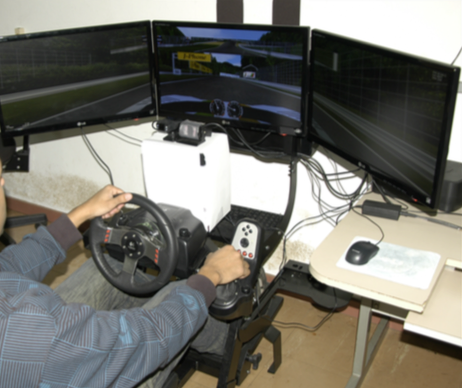
\includegraphics[width=0.3\textwidth]{foto1.png}
  \caption{Projeto de ADAS da UFOP num local virtual. Fonte: \cite{kitt}.}
  \label{fig:naoponderado}
\end{figure}

\section{Proposta de Pesquisa para Dissertação}

A proposta aqui apresentada é o desenvolvimento de um ADAS numa plataforma reconfigurável para análise de desempenho com ou outros sistemas desenvolvidos.

\newpage

\section*{\textit{Jornals} e Conferências}

{\it 
	\begin{itemize}
		\item \textbf{A2} ACM/SIGDA International Symposium on Field-Programmable Gate Arrays;
		\item \textbf{A2} International Conference on Field Programmable Logic and Applications;
		\item \textbf{B3} ACM Transactions on Reconfigurable Technology and Systems;
		\item \textbf{B3} International Conference on Engineering of Reconfigurable Systems and Algorithms (ERSA);
		\item \textbf{B3} Reconfigurable Architectures Workshop (RAW);
		\item \textbf{B4} International Conference on Reconfigurable Computing and FPGAs (ReConFig);
		\item \textbf{B4} International Journal of Reconfigurable Computing (Print)
		\item \textbf{B4} International Workshop on Reconfigurable Communication-centric Systems-on-Chip (ReCoSoC);
		\item \textbf{--} International Workshop on Applied Renconfigurable Computing (ARC);
		\item \textbf{--} International Workshop on Distributed Auto-Adaptive and Reconfigurable Systems (DARES@ICDCS);
		\item \textbf{--} International Workshop on High-Performance Renconfigurable Computing Technology and Applications (HPRTCA@SC);
		\item \textbf{--} International IEEE Symposium on Field-Programmable Custom Computing Machines;
		\item \textbf{--} International Conference on Field-Programmable Technology;
	\end{itemize}
}


\bibliographystyle{sbc}
\bibliography{sbc-template}

\end{document}
